\documentclass[tikz,border=2pt]{standalone}
\usepackage{fontspec}
\setmainfont{texgyreheros}[Extension=.otf,UprightFont=*-regular,BoldFont=*-bold,ItalicFont=*-italic]
\renewcommand{\familydefault}{\rmdefault}
\usepackage{amsmath}
\usetikzlibrary{arrows.meta,calc,positioning}
\begin{document}
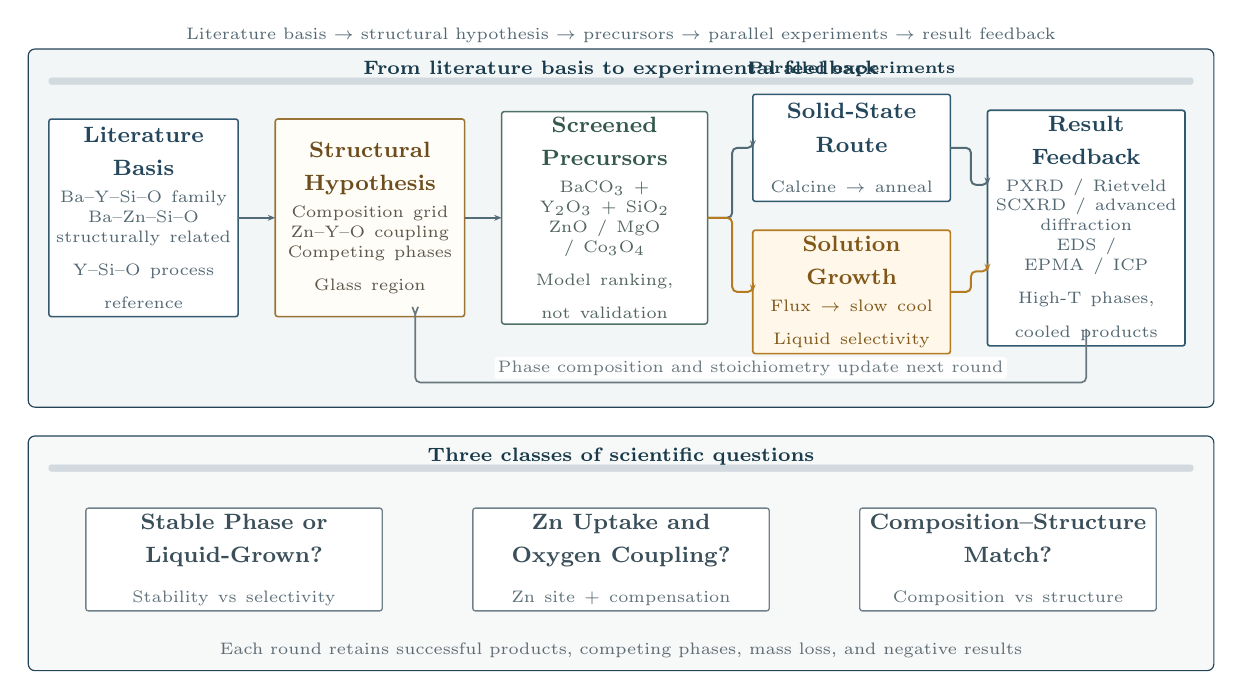
\begin{tikzpicture}[x=1pt,y=1pt, every node/.style={inner sep=0pt}]
\definecolor{gf}{HTML}{F3F6F7}\definecolor{gs}{HTML}{234456}
\filldraw[fill=gf, draw=gs, line width=0.42pt, rounded corners=2.4pt] (8.93pt,239.50pt) rectangle (437.34pt,110.08pt);
\definecolor{gf}{HTML}{F7F8F8}\definecolor{gs}{HTML}{234456}
\filldraw[fill=gf, draw=gs, line width=0.42pt, rounded corners=2.4pt] (8.93pt,99.67pt) rectangle (437.34pt,14.88pt);
\definecolor{nf}{HTML}{D3DADF}\definecolor{ns}{HTML}{D3DADF}
\filldraw[fill=nf, draw=ns, line width=0.15pt, rounded corners=0.9pt] (16.36pt,229.08pt) rectangle (429.90pt,226.70pt);
\definecolor{nf}{HTML}{D3DADF}\definecolor{ns}{HTML}{D3DADF}
\filldraw[fill=nf, draw=ns, line width=0.15pt, rounded corners=0.9pt] (16.36pt,89.25pt) rectangle (429.90pt,86.87pt);
\definecolor{nf}{HTML}{FFFFFF}\definecolor{ns}{HTML}{315A70}
\definecolor{lc}{HTML}{24475C}\definecolor{sc}{HTML}{536873}
\node[draw=ns, fill=nf, line width=0.54pt, rounded corners=0.9pt, minimum width=68.4pt, minimum height=71.4pt, text width=63.4pt, align=center, inner sep=2pt, anchor=center, text opacity=0] at (50.58pt,178.51pt) {\hyphenpenalty=9000\exhyphenpenalty=9000\relax {\bfseries\fontsize{8.0}{9.5}\selectfont\color{lc}Literature Basis}\\[2.4pt]{\fontsize{6.0}{7.2}\selectfont\color{sc}Ba--Y--Si--O family\\Ba--Zn--Si--O structurally related\\Y--Si--O process reference}};
\definecolor{nf}{HTML}{FFFDF7}\definecolor{ns}{HTML}{9A7436}
\definecolor{lc}{HTML}{6D4D1E}\definecolor{sc}{HTML}{5C554A}
\node[draw=ns, fill=nf, line width=0.57pt, rounded corners=0.9pt, minimum width=68.4pt, minimum height=71.4pt, text width=63.4pt, align=center, inner sep=2pt, anchor=center, text opacity=0] at (132.39pt,178.51pt) {\hyphenpenalty=9000\exhyphenpenalty=9000\relax {\bfseries\fontsize{8.0}{9.5}\selectfont\color{lc}Structural Hypothesis}\\[2.4pt]{\fontsize{6.0}{7.2}\selectfont\color{sc}Composition grid\\Zn--Y--O coupling\\Competing phases\\Glass region}};
\definecolor{nf}{HTML}{FFFFFF}\definecolor{ns}{HTML}{4D7165}
\definecolor{lc}{HTML}{34584C}\definecolor{sc}{HTML}{52655E}
\node[draw=ns, fill=nf, line width=0.54pt, rounded corners=0.9pt, minimum width=74.4pt, minimum height=71.4pt, text width=69.4pt, align=center, inner sep=2pt, anchor=center, text opacity=0] at (217.18pt,178.51pt) {\hyphenpenalty=9000\exhyphenpenalty=9000\relax {\bfseries\fontsize{8.0}{9.5}\selectfont\color{lc}Screened Precursors}\\[2.4pt]{\fontsize{6.0}{7.2}\selectfont\color{sc}BaCO$_{3}$ + Y$_{2}$O$_{3}$ + SiO$_{2}$\\ZnO / MgO / Co$_{3}$O$_{4}$\\Model ranking, not validation}};
\definecolor{nf}{HTML}{FFFFFF}\definecolor{ns}{HTML}{315A70}
\definecolor{lc}{HTML}{24475C}\definecolor{sc}{HTML}{536873}
\node[draw=ns, fill=nf, line width=0.54pt, rounded corners=0.9pt, minimum width=71.4pt, minimum height=38.7pt, text width=66.4pt, align=center, inner sep=2pt, anchor=center, text opacity=0] at (306.44pt,203.80pt) {\hyphenpenalty=9000\exhyphenpenalty=9000\relax {\bfseries\fontsize{8.0}{9.5}\selectfont\color{lc}Solid-State Route}\\[2.4pt]{\fontsize{6.0}{7.2}\selectfont\color{sc}Calcine $\rightarrow$ anneal}};
\definecolor{nf}{HTML}{FFF8EA}\definecolor{ns}{HTML}{B67A21}
\definecolor{lc}{HTML}{805718}\definecolor{sc}{HTML}{805718}
\node[draw=ns, fill=nf, line width=0.60pt, rounded corners=0.9pt, minimum width=71.4pt, minimum height=44.6pt, text width=66.4pt, align=center, inner sep=2pt, anchor=center, text opacity=0] at (306.44pt,151.73pt) {\hyphenpenalty=9000\exhyphenpenalty=9000\relax {\bfseries\fontsize{8.0}{9.5}\selectfont\color{lc}Solution Growth}\\[2.4pt]{\fontsize{6.0}{7.2}\selectfont\color{sc}Flux $\rightarrow$ slow cool\\Liquid selectivity}};
\definecolor{nf}{HTML}{FFFFFF}\definecolor{ns}{HTML}{315A70}
\definecolor{lc}{HTML}{24475C}\definecolor{sc}{HTML}{536873}
\node[draw=ns, fill=nf, line width=0.60pt, rounded corners=0.9pt, minimum width=71.4pt, minimum height=72.9pt, text width=66.4pt, align=center, inner sep=2pt, anchor=center, text opacity=0] at (391.23pt,174.79pt) {\hyphenpenalty=9000\exhyphenpenalty=9000\relax {\bfseries\fontsize{8.0}{9.5}\selectfont\color{lc}Result Feedback}\\[2.4pt]{\fontsize{6.0}{7.2}\selectfont\color{sc}PXRD / Rietveld\\SCXRD / advanced diffraction\\EDS / EPMA / ICP\\High-T phases, cooled products}};
\definecolor{nf}{HTML}{FFFFFF}\definecolor{ns}{HTML}{71818A}
\definecolor{lc}{HTML}{3A4F59}\definecolor{sc}{HTML}{61727B}
\node[draw=ns, fill=nf, line width=0.48pt, rounded corners=0.9pt, minimum width=107.1pt, minimum height=35.7pt, text width=102.1pt, align=center, inner sep=2pt, anchor=center, text opacity=0] at (83.30pt,55.04pt) {\hyphenpenalty=9000\exhyphenpenalty=9000\relax {\bfseries\fontsize{8.0}{9.5}\selectfont\color{lc}Stable Phase or Liquid-Grown?}\\[2.4pt]{\fontsize{6.0}{7.2}\selectfont\color{sc}Stability vs selectivity}};
\definecolor{nf}{HTML}{FFFFFF}\definecolor{ns}{HTML}{71818A}
\definecolor{lc}{HTML}{3A4F59}\definecolor{sc}{HTML}{61727B}
\node[draw=ns, fill=nf, line width=0.48pt, rounded corners=0.9pt, minimum width=107.1pt, minimum height=35.7pt, text width=102.1pt, align=center, inner sep=2pt, anchor=center, text opacity=0] at (223.13pt,55.04pt) {\hyphenpenalty=9000\exhyphenpenalty=9000\relax {\bfseries\fontsize{8.0}{9.5}\selectfont\color{lc}Zn Uptake and Oxygen Coupling?}\\[2.4pt]{\fontsize{6.0}{7.2}\selectfont\color{sc}Zn site + compensation}};
\definecolor{nf}{HTML}{FFFFFF}\definecolor{ns}{HTML}{71818A}
\definecolor{lc}{HTML}{3A4F59}\definecolor{sc}{HTML}{61727B}
\node[draw=ns, fill=nf, line width=0.48pt, rounded corners=0.9pt, minimum width=107.1pt, minimum height=35.7pt, text width=102.1pt, align=center, inner sep=2pt, anchor=center, text opacity=0] at (362.96pt,55.04pt) {\hyphenpenalty=9000\exhyphenpenalty=9000\relax {\bfseries\fontsize{8.0}{9.5}\selectfont\color{lc}Composition--Structure Match?}\\[2.4pt]{\fontsize{6.0}{7.2}\selectfont\color{sc}Composition vs structure}};
\definecolor{ec}{HTML}{536B77}
\draw[draw=ec, line width=0.77pt, -{Stealth[length=2.7pt,width=2.1pt]}, rounded corners=1.8pt] (84.79pt,178.51pt) -- (98.18pt,178.51pt);
\definecolor{ec}{HTML}{536B77}
\draw[draw=ec, line width=0.77pt, -{Stealth[length=2.7pt,width=2.1pt]}, rounded corners=1.8pt] (166.61pt,178.51pt) -- (179.99pt,178.51pt);
\definecolor{ec}{HTML}{536B77}
\draw[draw=ec, line width=0.71pt, -{Stealth[length=2.7pt,width=2.1pt]}, rounded corners=1.8pt] (254.37pt,178.51pt) -- (263.30pt,178.51pt) -- (263.30pt,203.80pt) -- (270.74pt,203.80pt) -- (270.74pt,203.80pt);
\definecolor{ec}{HTML}{B67A21}
\draw[draw=ec, line width=0.71pt, -{Stealth[length=2.7pt,width=2.1pt]}, rounded corners=1.8pt] (254.37pt,178.51pt) -- (263.30pt,178.51pt) -- (263.30pt,151.73pt) -- (270.74pt,151.73pt) -- (270.74pt,151.73pt);
\definecolor{ec}{HTML}{536B77}
\draw[draw=ec, line width=0.71pt, -{Stealth[length=2.7pt,width=2.1pt]}, rounded corners=1.8pt] (342.14pt,203.80pt) -- (349.58pt,203.80pt) -- (349.58pt,190.41pt) -- (355.53pt,190.41pt) -- (355.53pt,190.41pt);
\definecolor{ec}{HTML}{B67A21}
\draw[draw=ec, line width=0.71pt, -{Stealth[length=2.7pt,width=2.1pt]}, rounded corners=1.8pt] (342.14pt,151.73pt) -- (349.58pt,151.73pt) -- (349.58pt,159.17pt) -- (355.53pt,159.17pt) -- (355.53pt,159.17pt);
\definecolor{ec}{HTML}{69777E}
\draw[draw=ec, line width=0.60pt, -{Straight Barb[length=2.7pt,width=2.1pt]}, rounded corners=1.8pt] (391.23pt,138.34pt) -- (391.23pt,119.00pt) -- (148.76pt,119.00pt) -- (148.76pt,142.81pt) -- (148.76pt,142.81pt);
\node[fill=white, fill opacity=0.92, text opacity=1, inner sep=1.2pt, rounded corners=1pt, font=\fontsize{6.0}{6.7}\selectfont, text=ec, anchor=south, align=center] at (269.99pt,120.19pt) {Phase composition and stoichiometry update next round};
\definecolor{lc}{HTML}{24475C}\definecolor{sc}{HTML}{536873}
\node[minimum width=68.4pt, minimum height=71.4pt, text width=63.4pt, align=center, inner sep=2pt, anchor=center] at (50.58pt,178.51pt) {\hyphenpenalty=9000\exhyphenpenalty=9000\relax {\bfseries\fontsize{8.0}{9.5}\selectfont\color{lc}Literature Basis}\\[2.4pt]{\fontsize{6.0}{7.2}\selectfont\color{sc}Ba--Y--Si--O family\\Ba--Zn--Si--O structurally related\\Y--Si--O process reference}};
\definecolor{lc}{HTML}{6D4D1E}\definecolor{sc}{HTML}{5C554A}
\node[minimum width=68.4pt, minimum height=71.4pt, text width=63.4pt, align=center, inner sep=2pt, anchor=center] at (132.39pt,178.51pt) {\hyphenpenalty=9000\exhyphenpenalty=9000\relax {\bfseries\fontsize{8.0}{9.5}\selectfont\color{lc}Structural Hypothesis}\\[2.4pt]{\fontsize{6.0}{7.2}\selectfont\color{sc}Composition grid\\Zn--Y--O coupling\\Competing phases\\Glass region}};
\definecolor{lc}{HTML}{34584C}\definecolor{sc}{HTML}{52655E}
\node[minimum width=74.4pt, minimum height=71.4pt, text width=69.4pt, align=center, inner sep=2pt, anchor=center] at (217.18pt,178.51pt) {\hyphenpenalty=9000\exhyphenpenalty=9000\relax {\bfseries\fontsize{8.0}{9.5}\selectfont\color{lc}Screened Precursors}\\[2.4pt]{\fontsize{6.0}{7.2}\selectfont\color{sc}BaCO$_{3}$ + Y$_{2}$O$_{3}$ + SiO$_{2}$\\ZnO / MgO / Co$_{3}$O$_{4}$\\Model ranking, not validation}};
\definecolor{lc}{HTML}{24475C}\definecolor{sc}{HTML}{536873}
\node[minimum width=71.4pt, minimum height=38.7pt, text width=66.4pt, align=center, inner sep=2pt, anchor=center] at (306.44pt,203.80pt) {\hyphenpenalty=9000\exhyphenpenalty=9000\relax {\bfseries\fontsize{8.0}{9.5}\selectfont\color{lc}Solid-State Route}\\[2.4pt]{\fontsize{6.0}{7.2}\selectfont\color{sc}Calcine $\rightarrow$ anneal}};
\definecolor{lc}{HTML}{805718}\definecolor{sc}{HTML}{805718}
\node[minimum width=71.4pt, minimum height=44.6pt, text width=66.4pt, align=center, inner sep=2pt, anchor=center] at (306.44pt,151.73pt) {\hyphenpenalty=9000\exhyphenpenalty=9000\relax {\bfseries\fontsize{8.0}{9.5}\selectfont\color{lc}Solution Growth}\\[2.4pt]{\fontsize{6.0}{7.2}\selectfont\color{sc}Flux $\rightarrow$ slow cool\\Liquid selectivity}};
\definecolor{lc}{HTML}{24475C}\definecolor{sc}{HTML}{536873}
\node[minimum width=71.4pt, minimum height=72.9pt, text width=66.4pt, align=center, inner sep=2pt, anchor=center] at (391.23pt,174.79pt) {\hyphenpenalty=9000\exhyphenpenalty=9000\relax {\bfseries\fontsize{8.0}{9.5}\selectfont\color{lc}Result Feedback}\\[2.4pt]{\fontsize{6.0}{7.2}\selectfont\color{sc}PXRD / Rietveld\\SCXRD / advanced diffraction\\EDS / EPMA / ICP\\High-T phases, cooled products}};
\definecolor{lc}{HTML}{3A4F59}\definecolor{sc}{HTML}{61727B}
\node[minimum width=107.1pt, minimum height=35.7pt, text width=102.1pt, align=center, inner sep=2pt, anchor=center] at (83.30pt,55.04pt) {\hyphenpenalty=9000\exhyphenpenalty=9000\relax {\bfseries\fontsize{8.0}{9.5}\selectfont\color{lc}Stable Phase or Liquid-Grown?}\\[2.4pt]{\fontsize{6.0}{7.2}\selectfont\color{sc}Stability vs selectivity}};
\definecolor{lc}{HTML}{3A4F59}\definecolor{sc}{HTML}{61727B}
\node[minimum width=107.1pt, minimum height=35.7pt, text width=102.1pt, align=center, inner sep=2pt, anchor=center] at (223.13pt,55.04pt) {\hyphenpenalty=9000\exhyphenpenalty=9000\relax {\bfseries\fontsize{8.0}{9.5}\selectfont\color{lc}Zn Uptake and Oxygen Coupling?}\\[2.4pt]{\fontsize{6.0}{7.2}\selectfont\color{sc}Zn site + compensation}};
\definecolor{lc}{HTML}{3A4F59}\definecolor{sc}{HTML}{61727B}
\node[minimum width=107.1pt, minimum height=35.7pt, text width=102.1pt, align=center, inner sep=2pt, anchor=center] at (362.96pt,55.04pt) {\hyphenpenalty=9000\exhyphenpenalty=9000\relax {\bfseries\fontsize{8.0}{9.5}\selectfont\color{lc}Composition--Structure Match?}\\[2.4pt]{\fontsize{6.0}{7.2}\selectfont\color{sc}Composition vs structure}};
\definecolor{tc}{HTML}{536873}
\node[anchor=center, font=\fontsize{6.1}{7.4}\selectfont, text=tc] at (223.13pt,244.55pt) {Literature basis $\rightarrow$ structural hypothesis $\rightarrow$ precursors $\rightarrow$ parallel experiments $\rightarrow$ result feedback};
\definecolor{tc}{HTML}{183A4A}
\node[anchor=center, font=\bfseries\fontsize{7.2}{8.7}\selectfont, text=tc] at (223.13pt,232.06pt) {From literature basis to experimental feedback};
\definecolor{tc}{HTML}{183A4A}
\node[anchor=center, font=\bfseries\fontsize{6.5}{7.8}\selectfont, text=tc] at (306.44pt,232.06pt) {Parallel experiments};
\definecolor{tc}{HTML}{183A4A}
\node[anchor=center, font=\bfseries\fontsize{7.2}{8.7}\selectfont, text=tc] at (223.13pt,92.23pt) {Three classes of scientific questions};
\definecolor{tc}{HTML}{5F6B73}
\node[anchor=center, font=\fontsize{6.1}{7.4}\selectfont, text=tc] at (223.13pt,22.31pt) {Each round retains successful products, competing phases, mass loss, and negative results};
\end{tikzpicture}
\end{document}